\section{Introducción}

\subsection{Motivación y Problemática}

Uno de los desafíos persistentes que surge al analizar el despliegue de Smart Cities radica en la brecha creciente entre las demandas de monitoreo ubicuo y la cobertura real que ofrecen las redes terrestres convencionales. Aunque las infraestructuras 5G han avanzado notablemente en entornos urbanos densos, persisten zonas de sombra significativas: periferias metropolitanas, corredores de transporte elevados y áreas densamente pobladas donde la interferencia y la saturación limitan el rendimiento de miles de dispositivos IoT. 

Resulta revelador observar cómo, en muchos casos estudiados, las redes puramente terrestres (TN) tienden a fallar precisamente cuando más se necesitan: durante picos de demanda o ante fallos en la infraestructura crítica. Un survey exhaustivo sobre LPWAN e IoT en entornos urbanos \cite{Ogbodo2022} pone de manifiesto estas limitaciones estructurales, destacando que incluso tecnologías maduras como NB-IoT enfrentan problemas de escalabilidad y cobertura completa. 

Particularmente llamativo es el potencial que muestran las Redes No Terrestres (NTN) para complementar estas carencias. Lejos de ser una solución marginal, la coexistencia TN-NTN emerge como elemento clave en la evolución hacia 6G, especialmente en lo que respecta a handover seamless y soporte a ultra-dense IoT deployments \cite{Alsaeedy2025}. No obstante, cabe matizar que la integración efectiva dista de ser trivial: desafíos de latencia variable, gestión de recursos compartidos y mecanismos de conmutación robustos siguen requiriendo atención cuidadosa.

\begin{table}[t]
\centering
\caption{Comparación entre Redes Terrestres (TN) y No Terrestres (NTN) en contexto de aplicaciones IoT para Smart Cities}
\label{tab:tn_vs_ntn}
\begin{tabular}{lcc}
\hline
\textbf{Métrica} & \textbf{TN} & \textbf{NTN} \\
\hline
Cobertura & Limitada a zonas urbanas densas & Global, incluyendo áreas remotas \\
Latencia típica & 1--10 ms & 10--600 ms (según órbita) \\
Confiabilidad en movilidad & Alta en cobertura & Variable, depende de visibilidad \\
Densidad de dispositivos & Muy alta en celda & Media-alta (limitada por bandwidth) \\
Consumo energético (dispositivos) & Bajo-moderado & Moderado (mayor en uplinks largos) \\
Resiliencia ante desastres & Baja & Alta \\
\hline
\end{tabular}
\end{table}

\subsection{Contribuciones Principales}

Frente a este panorama, el presente trabajo propone una arquitectura de integración híbrida sat-terrestre específicamente optimizada para monitoreo inteligente en Smart Cities. Más allá de una simple superposición de tecnologías, el framework desarrollado habilita conectividad multi-enlace dinámica que combina lo mejor de ambos mundos: la baja latencia y alta capacidad terrestre con la cobertura ubicua y resiliencia de los segmentos NTN.

Aunque existen iniciativas previas interesantes, como el uso de globos de gran altitud para extender conectividad IoT urbana \cite{Prathiba2024}, nuestra propuesta avanza hacia un modelo más maduro de multi-conectividad gestionada de forma inteligente. Entre las contribuciones centrales destacan: el diseño de un esquema de handover contextual basado en métricas de aplicación, un modelo analítico para predecir rendimiento híbrido en escenarios de monitoreo (tráfico, calidad ambiental e infraestructura crítica), y una evaluación cuantitativa que demuestra mejoras sustanciales en cobertura efectiva y eficiencia energética.

\begin{figure}[t]
\centering
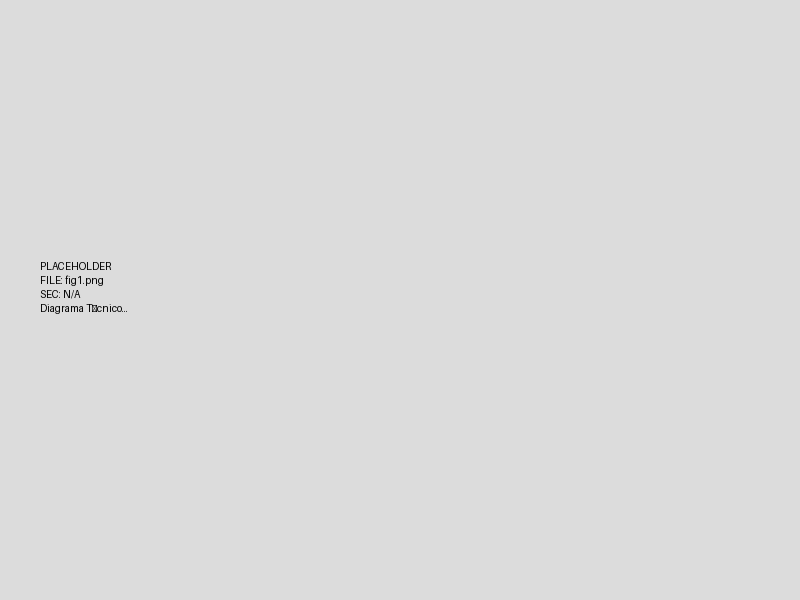
\includegraphics[width=\linewidth]{fig1.png}
\caption{Arquitectura general híbrida TN-NTN para IoT en Smart Cities, mostrando capas de conectividad terrestre, LEO y GEO junto con flujos de datos de monitoreo.}
\label{fig:arquitectura_hibrida}
\end{figure}

\subsection{Organización del Documento}

El resto del artículo se estructura de manera que guía al lector desde los fundamentos teóricos hasta la validación práctica. La Sección 2 revisa el estado del arte en NTN-IoT y su aplicación en entornos urbanos. Posteriormente, la Sección 3 detalla la arquitectura propuesta, con énfasis en los mecanismos de integración y gestión de recursos. Las Secciones 4 y 5 presentan la metodología de evaluación y los resultados obtenidos, respectivamente, mientras que la Sección 6 discute implicaciones, limitaciones y comparaciones. Finalmente, la Sección 7 sintetiza conclusiones y traza líneas de trabajo futuro.

Esta organización busca no solo exponer una solución técnica, sino también ofrecer insights accionables para investigadores y despliegues reales en ciudades del mañana.